\documentclass[tikz,border=8pt]{standalone}
\usepackage[T1]{fontenc}
\usepackage{lmodern}
\usepackage{tikz}
\usetikzlibrary{arrows.meta}

\definecolor{ink}{HTML}{243447}
\definecolor{bluefill}{HTML}{EAF3FB}
\definecolor{purplefill}{HTML}{F3EDFA}
\definecolor{greenfill}{HTML}{EDF6EB}
\definecolor{yellowfill}{HTML}{FFF3D9}
\definecolor{tealfill}{HTML}{E8F7F3}

\tikzset{
  flow/.style={-{Latex[length=2.2mm]},draw=ink!75,line width=.8pt,rounded corners=2pt},
  optional/.style={flow,densely dashed},
  lane/.style={draw=ink!75,line width=.8pt,rounded corners=5pt},
  stagebox/.style={draw=ink!70,fill=white,rounded corners=3pt,line width=.65pt,
    minimum height=.82cm,text width=5.9cm,inner sep=4pt,align=left,font=\sffamily\small},
  mini/.style={draw=ink!70,fill=white,rounded corners=3pt,line width=.65pt,
    minimum height=.92cm,text width=2.65cm,inner sep=4pt,align=center,font=\sffamily\scriptsize}
}

\newcommand{\stepbox}[5]{%
  \node[stagebox,anchor=north west] (#1) at (#2,#3)
    {\textbf{#4}\\[-1pt]{\scriptsize #5}};
}

\begin{document}
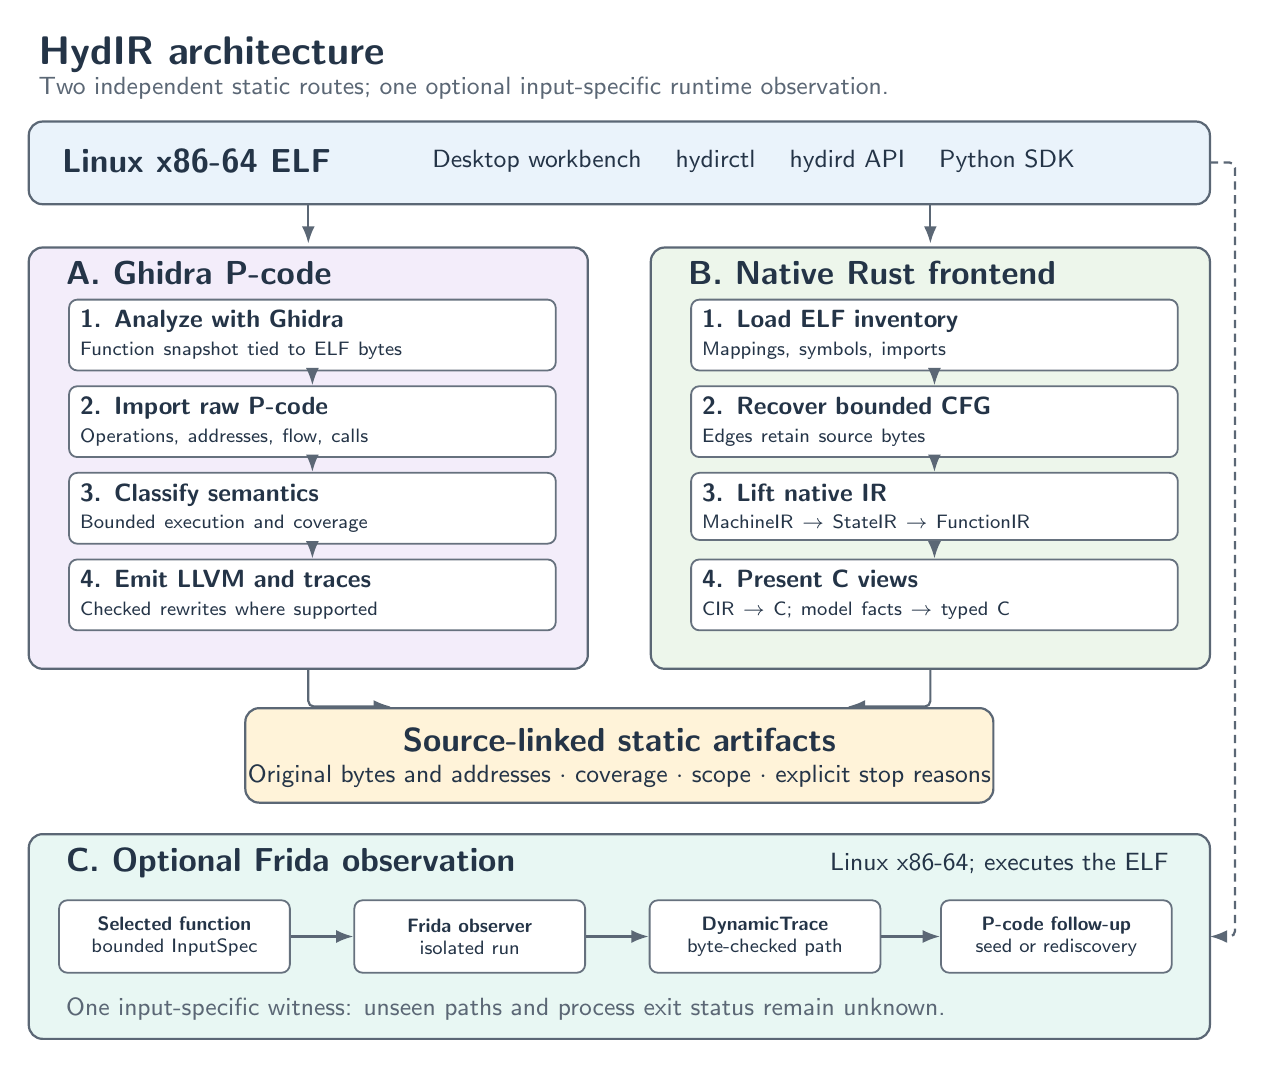
\begin{tikzpicture}[x=1cm,y=-1cm,every node/.style={text=ink}]
  \node[anchor=west,font=\sffamily\bfseries\Large] at (.5,.45)
    {HydIR architecture};
  \node[anchor=west,font=\sffamily\small,text=ink!75] at (.5,.88)
    {Two independent static routes; one optional input-specific runtime observation.};

  % Input and interfaces.
  \draw[lane,fill=bluefill] (.5,1.3) rectangle (15.5,2.35);
  \node[anchor=west,font=\sffamily\bfseries\large] at (.8,1.8)
    {Linux x86-64 ELF};
  \node[anchor=west,font=\sffamily\small] at (5.5,1.8)
    {Desktop workbench \quad hydirctl \quad hydird API \quad Python SDK};
  \draw[flow] (4.05,2.35) -- (4.05,2.85);
  \draw[flow] (11.95,2.35) -- (11.95,2.85);

  % Ghidra P-code lane.
  \draw[lane,fill=purplefill] (.5,2.9) rectangle (7.6,8.25);
  \node[anchor=west,font=\sffamily\bfseries\large] at (.85,3.22)
    {A. Ghidra P-code};
  \stepbox{g1}{1.0}{3.55}{1. Analyze with Ghidra}{Function snapshot tied to ELF bytes}
  \stepbox{g2}{1.0}{4.65}{2. Import raw P-code}{Operations, addresses, flow, calls}
  \stepbox{g3}{1.0}{5.75}{3. Classify semantics}{Bounded execution and coverage}
  \stepbox{g4}{1.0}{6.85}{4. Emit LLVM and traces}{Checked rewrites where supported}
  \draw[flow] (g1.south) -- (g2.north);
  \draw[flow] (g2.south) -- (g3.north);
  \draw[flow] (g3.south) -- (g4.north);

  % Independent native lane.
  \draw[lane,fill=greenfill] (8.4,2.9) rectangle (15.5,8.25);
  \node[anchor=west,font=\sffamily\bfseries\large] at (8.75,3.22)
    {B. Native Rust frontend};
  \stepbox{n1}{8.9}{3.55}{1. Load ELF inventory}{Mappings, symbols, imports}
  \stepbox{n2}{8.9}{4.65}{2. Recover bounded CFG}{Edges retain source bytes}
  \stepbox{n3}{8.9}{5.75}{3. Lift native IR}{MachineIR $\to$ StateIR $\to$ FunctionIR}
  \stepbox{n4}{8.9}{6.85}{4. Present C views}{CIR $\to$ C; model facts $\to$ typed C}
  \draw[flow] (n1.south) -- (n2.north);
  \draw[flow] (n2.south) -- (n3.north);
  \draw[flow] (n3.south) -- (n4.north);

  % Shared contract for the two static routes.
  \draw[flow] (4.05,8.25) |- (5.1,8.73);
  \draw[flow] (11.95,8.25) |- (10.9,8.73);
  \draw[lane,fill=yellowfill] (3.25,8.75) rectangle (12.75,9.95);
  \node[align=center,font=\sffamily\bfseries\large] at (8,9.15)
    {Source-linked static artifacts};
  \node[align=center,font=\sffamily\small] at (8,9.62)
    {Original bytes and addresses $\cdot$ coverage $\cdot$ scope $\cdot$ explicit stop reasons};

  % Frida runs the input ELF and only witnesses the selected input path.
  \draw[optional] (15.5,1.82) -- (15.82,1.82) -- (15.82,11.65) -- (15.5,11.65);
  \draw[lane,fill=tealfill] (.5,10.35) rectangle (15.5,12.95);
  \node[anchor=west,font=\sffamily\bfseries\large] at (.85,10.72)
    {C. Optional Frida observation};
  \node[anchor=east,font=\sffamily\small] at (15.1,10.72)
    {Linux x86-64; executes the ELF};
  \node[mini] (f1) at (2.35,11.65)
    {\textbf{Selected function}\\bounded InputSpec};
  \node[mini] (f2) at (6.1,11.65)
    {\textbf{Frida observer}\\isolated run};
  \node[mini] (f3) at (9.85,11.65)
    {\textbf{DynamicTrace}\\byte-checked path};
  \node[mini] (f4) at (13.55,11.65)
    {\textbf{P-code follow-up}\\seed or rediscovery};
  \draw[flow] (f1.east) -- (f2.west);
  \draw[flow] (f2.east) -- (f3.west);
  \draw[flow] (f3.east) -- (f4.west);
  \node[anchor=west,font=\sffamily\small,text=ink!75] at (.85,12.58)
    {One input-specific witness: unseen paths and process exit status remain unknown.};
\end{tikzpicture}
\end{document}
